%=============================================================================
% RAPPORT PFE — Maintenance Prédictive des Roulements Industriels
% Auteur : Mohamed Yassine Balti — ISG Bizerte / Novation City
% Version corrigée : conforme au code source réel (juin 2026)
%=============================================================================

\documentclass[12pt,a4paper]{report}

% ── Encodage et langue ────────────────────────────────────────────────────────
\usepackage[utf8]{inputenc}
\usepackage[T1]{fontenc}
\usepackage[french]{babel}

% ── Mise en page ──────────────────────────────────────────────────────────────
\usepackage[top=2.5cm,bottom=2.5cm,left=3cm,right=2.5cm]{geometry}
\usepackage{setspace}
\onehalfspacing

% ── Graphiques et couleurs ────────────────────────────────────────────────────
\usepackage{graphicx}
\usepackage[table,xcdraw]{xcolor}
\usepackage{tikz}
\usepackage{pgfplots}
\pgfplotsset{compat=1.18}

% ── Tableaux ──────────────────────────────────────────────────────────────────
\usepackage{booktabs}
\usepackage{longtable}
\usepackage{array}
\usepackage{multirow}
\usepackage{tabularx}
\usepackage{makecell}

% ── Mathématiques ─────────────────────────────────────────────────────────────
\usepackage{amsmath,amssymb,amsfonts}

% ── Code source ───────────────────────────────────────────────────────────────
\usepackage{listings}
\lstset{
  basicstyle=\small\ttfamily,
  breaklines=true,
  frame=single,
  backgroundcolor=\color{gray!8}
}

% ── Liens hypertexte ──────────────────────────────────────────────────────────
\usepackage[hidelinks,colorlinks=false]{hyperref}

% ── En-têtes / pieds de page ──────────────────────────────────────────────────
\usepackage{fancyhdr}
\pagestyle{fancy}
\fancyhf{}
\fancyhead[L]{\small Maintenance Prédictive des Roulements}
\fancyhead[R]{\small \thepage}
\fancyfoot[C]{\small ISG Bizerte | Novation City | 2025--2026}
\renewcommand{\headrulewidth}{0.4pt}

% ── Couleurs thématiques ──────────────────────────────────────────────────────
\definecolor{darkblue}{RGB}{26,56,96}
\definecolor{lightblue}{RGB}{173,216,230}
\definecolor{alertred}{RGB}{200,0,0}
\definecolor{alertorange}{RGB}{230,120,0}
\definecolor{alertyellow}{RGB}{200,180,0}
\definecolor{alertgreen}{RGB}{0,150,0}
\definecolor{codegray}{RGB}{240,240,240}

% ── Boîtes d'encadré ──────────────────────────────────────────────────────────
\usepackage{tcolorbox}
\tcbuselibrary{skins,breakable}
\newtcolorbox{correctionbox}{
  colback=yellow!10,colframe=orange!80!black,
  title={\textbf{Correction apportée}},fonttitle=\bfseries
}

% ── Symboles check/cross ──────────────────────────────────────────────────────
\usepackage{pifont}
\newcommand{\cmark}{\ding{51}}
\newcommand{\xmark}{\ding{55}}

%=============================================================================
\begin{document}
%=============================================================================

%─────────────────────────────────────────────────────────────────────────────
% PAGE DE TITRE
%─────────────────────────────────────────────────────────────────────────────
\begin{titlepage}
\centering
{\Large \textbf{République Tunisienne}}\par
{\large Ministère de l'Enseignement Supérieur et de la Recherche Scientifique}\par
\vspace{0.3cm}
{\Large \textbf{Université de Carthage}}\par
{\large Institut Supérieur de Gestion de Bizerte}\par
\vspace{1.5cm}
\textcolor{darkblue}{\rule{\linewidth}{1.5pt}}\par
\vspace{0.8cm}
{\LARGE \textbf{Projet de Fin d'Études}}\par
\vspace{0.5cm}
{\large Présenté à l'Institut Supérieur de Gestion de Bizerte}\par
{\large En vue de l'obtention de la Licence}\par
\vspace{0.8cm}
{\large Par}\par
\vspace{0.3cm}
{\Huge \textbf{\textcolor{darkblue}{Mohamed Yassine Balti}}}\par
\vspace{1cm}
\fcolorbox{darkblue}{darkblue!10}{
  \begin{minipage}{0.85\linewidth}
  \centering\vspace{0.4cm}
  {\Large \textbf{Conception et Réalisation d'un Système de}}\\[0.3cm]
  {\Large \textbf{Maintenance Prédictive des Roulements Industriels}}\\[0.3cm]
  {\Large \textbf{par Intelligence Artificielle}}\\[0.3cm]
  {\Large \textbf{avec Surveillance IoT}}\\[0.4cm]
  \end{minipage}
}\par
\vspace{1.5cm}
\begin{tabular}{ll}
\toprule
\textbf{Nom \& Prénom} & \textbf{Rôle} \\
\midrule
M./Mme [NOM PRÉSIDENT]      & Président \\
M./Mme [NOM RAPPORTEUR]     & Rapporteur \\
Mme Amel Hajji              & Encadrant Académique \\
M. Mohamed Chrifa           & Encadrant d'Entreprise \\
\bottomrule
\end{tabular}\par
\vfill
{\large Année universitaire \textbf{2025--2026}}
\end{titlepage}

%─────────────────────────────────────────────────────────────────────────────
\chapter*{Dédicaces}
\addcontentsline{toc}{chapter}{Dédicaces}

\begin{center}
\textit{« Qu'il me soit permis au sein de ce modeste projet\\
d'exprimer ma profonde reconnaissance à : »}
\end{center}

\textbf{Mon cher père Mustapha,}

Qui n'a jamais cessé de me soutenir et m'encourager. À qui je dois ma réussite,
aucun mot ne serait assez pour témoigner de l'étendue des sentiments que j'éprouve à
son égard.

\textbf{Ma chère mère Raoudha,}

Que nulle dédicace ne puisse exprimer ce que je lui dois pour son amour inépuisable,
sa sensibilité et sa patience, pour son immense affectation et sollicitude, ses sacrifices
et sa confiance durant mes études.

\textbf{À mes frères et sœurs,}

Asma, Mohamed Anis, Tarek, Safa et Yahya des personnes qui me sont très chères
et qui m'ont toujours apporté leur aide, qu'ils trouvent ici l'expression d'un amour sincère.

\textbf{À tous mes amis et camarades de promotion,}

Pour tous les moments partagés, les discussions enrichissantes et l'entraide précieuse
tout au long de cette formation.

\hfill \textit{Mohamed Yassine Balti}

%─────────────────────────────────────────────────────────────────────────────
\chapter*{Remerciements}
\addcontentsline{toc}{chapter}{Remerciements}

Au terme de ce travail, je tiens à exprimer ma profonde reconnaissance et mes vifs
remerciements à Mme la directrice de l'ISG BIZERTE et Mr le directeur de Novation
City nous avoir accueillis dans leurs établissements.

Je remercie également \textbf{Madame Amel Hajji}, mon encadrant de l'ISG de BIZERTE,
pour son soutien et ses précieux conseils afin de mener à bien ce projet.

Ma reconnaissance et ma gratitude vont vaillances à \textbf{Monsieur Mohamed Chrifa},
mon encadrant de Novation City, qui m'a aimablement guidé et prodigué de ses conseils
précieux au cours de mon projet de fin d'étude.

Je tiens aussi à être reconnaissant envers mes enseignants de l'ISG de BIZERTE pour
la formation qu'ils m'ont donnée. Je tiens également mes remerciements envers toute
l'équipe de Novation City pour leurs disponibilités.

\hfill \textit{Mohamed Yassine Balti}

%─────────────────────────────────────────────────────────────────────────────
\chapter*{Résumé}
\addcontentsline{toc}{chapter}{Résumé}

Ce projet de fin d'études porte sur la conception et la réalisation d'un système
complet de maintenance prédictive pour la surveillance de 20 capteurs IFM industriels
déployés sur les moteurs asynchrones de Novation City (Sousse, Tunisie).

Le système repose sur une chaîne de traitement intégrale : acquisition des données en
temps réel depuis une base de données MariaDB (polling toutes les 2~secondes via
\texttt{realtime\_mariadb.py}), ingénierie de \textbf{31 features} statistiques, temporelles,
fréquentielles (FFT, analyse spectrale) et d'accélération extraites sur une fenêtre
glissante $w=20$, normalisation par \texttt{RobustScaler}, réduction de dimension par
\textbf{PCA à 95\% de variance conservée}, puis inférence par un \textbf{ensemble de
6 modèles non supervisés} (Isolation Forest, LOF, OCSVM, ECOD, HBOS, COPOD)
combinés par \textbf{SoftVote à seuil dynamique optimal}.

Les modèles, entraînés sur 73\,917 sessions issues de 240\,000 mesures réelles IFM avec
une contamination de 20\%, atteignent une \textbf{AUC-ROC de 0,836} et un \textbf{Recall de 0,877},
ce qui garantit la détection de la très grande majorité des anomalies au prix d'une
précision conservative. La prédiction de la Durée de Vie Résiduelle (RUL) est assurée
par un \textbf{GradientBoostingRegressor} entraîné sur des courbes de dégradation
synthétiques (modèle de Weibull, $n=12\,000$) avec une MAE de 317~h et $R^2=0{,}56$.

L'ensemble est exposé par une \textbf{API REST FastAPI v3.1.0} (port 8000, 11 endpoints)
et visualisé via un \textbf{dashboard HTML5} se rafraîchissant toutes les 3~secondes.

\textbf{Mots-clés :} maintenance prédictive, IoT, IFM, détection d'anomalies non supervisée,
Isolation Forest, ECOD, HBOS, COPOD, RUL, GradientBoosting, FastAPI, MariaDB.

\tableofcontents
\listoffigures
\listoftables

%─────────────────────────────────────────────────────────────────────────────
\chapter*{Liste des Abréviations}
\addcontentsline{toc}{chapter}{Liste des Abréviations}

\begin{tabular}{p{2.5cm}p{10cm}}
\toprule
\textbf{Abréviation} & \textbf{Signification} \\
\midrule
IA     & Intelligence Artificielle \\
ML     & Machine Learning (Apprentissage Automatique) \\
RUL    & Remaining Useful Life (Durée de Vie Résiduelle) \\
IoT    & Internet of Things (Internet des Objets) \\
IF     & Isolation Forest \\
LOF    & Local Outlier Factor \\
OCSVM  & One-Class Support Vector Machine \\
ECOD   & Empirical Cumulative distribution-based Outlier Detection \\
HBOS   & Histogram-Based Outlier Score \\
COPOD  & Copula-Based Outlier Detection \\
AUC    & Area Under the Curve (Aire sous la courbe ROC) \\
ROC    & Receiver Operating Characteristic \\
MQTT   & Message Queuing Telemetry Transport \\
API    & Application Programming Interface \\
FFT    & Fast Fourier Transform (Transformée de Fourier Rapide) \\
BPFO   & Ball Pass Frequency Outer Race \\
BPFI   & Ball Pass Frequency Inner Race \\
BSF    & Ball Spin Frequency \\
FTF    & Fundamental Train Frequency \\
GBR    & GradientBoostingRegressor \\
PCA    & Principal Component Analysis \\
CSV    & Comma-Separated Values \\
RPi4   & Raspberry Pi 4 \\
\bottomrule
\end{tabular}

%=============================================================================
\chapter*{Introduction Générale}
\addcontentsline{toc}{chapter}{Introduction Générale}
%=============================================================================

De nos jours, la maintenance industrielle classique cède de plus en plus la place à la
maintenance prédictive, portée par l'essor de l'Intelligence Artificielle et de l'Internet
des Objets (IoT). Cette transition vise à transformer la gestion des équipements en
passant d'un mode réactif (réparer après la panne) à un mode proactif.

C'est dans ce cadre que notre projet vise à concevoir et mettre en place un système
complet de maintenance prédictive pour la surveillance de 20 capteurs IFM industriels
déployés sur les moteurs de Novation City. Le système fournit aux responsables de
maintenance une visibilité en temps réel sur l'état de santé de chaque moteur, un score
d'anomalie calculé en continu et une estimation de la durée de vie résiduelle (RUL)
en heures et en jours.

La solution repose sur l'acquisition des données en temps réel depuis une base de données
MariaDB via \texttt{realtime\_mariadb.py} (polling toutes les 2~secondes), un pipeline
d'ingénierie de \textbf{31 features} (statistiques temporelles, FFT, accélération, entropie),
et un ensemble de \textbf{6 modèles non supervisés} (Isolation Forest, LOF, OCSVM, ECOD,
HBOS, COPOD) combinés par SoftVote à seuil dynamique. Ces modèles, entraînés sur
73\,917 sessions avec une contamination de 20\%, atteignent une AUC-ROC de 0,836 et un
Recall de 0,877. La prédiction RUL est assurée par un GradientBoostingRegressor (MAE~=~317~h,
$R^2=0{,}56$). L'ensemble est exposé par une API REST FastAPI v3.1.0 (11 endpoints,
port 8000) et visualisé via un dashboard HTML5 natif se rafraîchissant toutes les 3~secondes.

Le présent rapport se compose de quatre chapitres :
\begin{itemize}
  \item Le \textbf{premier chapitre} présente le cadre général, l'étude de l'existant, la problématique et la méthodologie CRISP-DM.
  \item Le \textbf{deuxième chapitre} définit les objectifs métier et data science, l'état de l'art et la préparation des données.
  \item Le \textbf{troisième chapitre} expose l'architecture complète, la couche IoT (MariaDB temps réel), le pipeline ML à 6 modèles, le calcul du RUL par GBR, l'API FastAPI et le dashboard.
  \item Le \textbf{quatrième chapitre} présente l'évaluation, les performances réelles obtenues et les tests de bout en bout.
\end{itemize}

%=============================================================================
\chapter{Cadre du Projet}
%=============================================================================

\section{Introduction}

Dans ce chapitre, nous débutons par une présentation de l'organisme d'accueil et le
contexte global de notre projet. Nous identifierons ensuite la problématique principale
que ce projet vise à résoudre et détaillerons notre approche méthodologique.

\section{Présentation de l'organisme d'accueil}

Ce projet de fin d'études s'est déroulé au sein du pôle de compétitivité de Sousse,
\textbf{Novation City}. Véritable catalyseur d'innovation en Tunisie, Novation City a pour
vocation de structurer et de dynamiser l'écosystème régional en facilitant le rapprochement entre les entreprises (startups, PMEs), les centres de recherche et les établissements d'enseignement supérieur.

Sur le plan technique, l'organisme dispose d'un parc de 21 moteurs asynchrones
triphasés fonctionnant en régime continu. Ces moteurs, équipés de roulements à billes,
sont instrumentés par des capteurs IFM mesurant la température, les vibrations selon
trois axes (X, Y, Z) et le courant électrique. Les données sont centralisées dans une
base de données \textbf{MariaDB 10.4} nommée \texttt{ai\_cp}.

\section{Problématique}

Malgré la présence d'une infrastructure de surveillance basique, l'entreprise est
confrontée à des défaillances récurrentes et coûteuses de roulements. Ces défaillances
surviennent sous quatre formes caractéristiques (Tableau~\ref{tab:defauts_roulements}).

\begin{table}[h]
\centering
\caption{Types de défauts de roulements et fréquences caractéristiques}
\label{tab:defauts_roulements}
\begin{tabular}{lll}
\toprule
\textbf{Type de défaut} & \textbf{Fréquence} & \textbf{Description physique} \\
\midrule
Défaut de bille        & BSF  & Impulsions périodiques générées par la rotation \\
Défaut piste intérieure & BPFI & Choc au passage d'une bille sur l'écaillage \\
Défaut piste extérieure & BPFO & Le plus fréquent, détectable par analyse d'enveloppe \\
Défaut de cage         & FTF  & Fréquence basse, lié à la déformation de la cage \\
\bottomrule
\end{tabular}
\end{table}

\section{Étude de l'existant}

\subsection{La maintenance corrective}
La maintenance corrective consiste à n'intervenir qu'après la panne (\textit{run-to-failure}).
Le coût d'une telle intervention peut être de trois à cinq fois supérieur à celui d'une maintenance planifiée.

\subsection{La maintenance préventive calendaire}
Elle consiste à remplacer les composants à intervalles fixes, ignorant l'état réel de la machine.

\section{Solution proposée}

L'architecture de notre solution répond directement à la problématique identifiée.
La détection d'anomalies repose sur un \textbf{ensemble de six modèles non supervisés} :
Isolation Forest (IF), Local Outlier Factor (LOF), One-Class SVM (OCSVM), ECOD,
HBOS et COPOD, combinés par \textbf{SoftVote à seuil dynamique optimal}.

La prédiction de la Durée de Vie Résiduelle (RUL) est assurée par un
\textbf{GradientBoostingRegressor} (46 features, $n=12\,000$ exemples synthétiques
Weibull, MAE~test~$=317$~h, $R^2=0{,}56$).

Les données sont acquises en temps réel depuis \textbf{MariaDB} via le module
\texttt{realtime\_mariadb.py} (polling toutes les 2~secondes). Un mode \textbf{replay}
basé sur les données historiques est également disponible pour les tests sans base de données active.

\section{Méthodologie du projet}

\subsection{Présentation de CRISP-DM}

CRISP-DM est la méthodologie de fouille de données la plus largement adoptée.
Elle propose un processus itératif organisé en six phases (Tableau~\ref{tab:crispdm}).

\begin{table}[h]
\centering
\caption{Les six phases de CRISP-DM}
\label{tab:crispdm}
\begin{tabular}{clp{8cm}}
\toprule
\textbf{\#} & \textbf{Phase} & \textbf{Description} \\
\midrule
1 & Compréhension métier   & Définir les objectifs et critères de succès \\
2 & Compréhension données  & Explorer et évaluer la qualité des données \\
3 & Préparation des données & Nettoyer, transformer, construire les features \\
4 & Modélisation           & Sélectionner et appliquer les algorithmes ML \\
5 & Évaluation             & Valider que les modèles répondent aux objectifs \\
6 & Déploiement            & Mettre le système en production \\
\bottomrule
\end{tabular}
\end{table}

\subsection{Choix de la méthodologie}

Le choix de CRISP-DM se justifie par la nature fondamentalement \textit{data-driven}
du projet et son caractère itératif, qui a permis de passer de l'approche supervisée
initialement envisagée (CNN-LSTM) vers l'approche non supervisée à 6 modèles finalement retenue.

\section{Conclusion}

Ce premier chapitre a fourni une vue d'ensemble du cadre du projet. Le chapitre suivant
détaille la compréhension des objectifs métier et data science ainsi que la préparation des données.

%=============================================================================
\chapter{Compréhension des Objectifs}
%=============================================================================

\section{Introduction}

Ce chapitre couvre les trois composantes du système : la couche IoT (acquisition temps réel depuis MariaDB), le pipeline IA (31 features, 6 modèles, RUL par GBR) et le dashboard de visualisation.

\section{État de l'art}

\subsection{Tableau comparatif}

\begin{table}[h]
\centering
\caption{Comparaison des solutions de maintenance prédictive}
\label{tab:comparaison}
\begin{tabularx}{\textwidth}{Xcccc}
\toprule
\textbf{Critère} & \textbf{IBM Maximo} & \textbf{Siemens MindSphere} & \textbf{Notre solution} \\
\midrule
Apprentissage non supervisé   & \xmark & \xmark & \cmark \\
6 modèles ensemble + SoftVote  & \xmark & \xmark & \cmark \\
RUL par modèle ML dédié (GBR) & Partiel & Partiel & \cmark \\
Features spectrales (FFT)      & \cmark & \cmark & \cmark \\
Déploiement on-premise         & Partiel & \xmark & \cmark \\
Compatibilité MariaDB native   & \xmark & \xmark & \cmark \\
Accessibilité financière (PME) & \xmark & \xmark & \cmark \\
\bottomrule
\end{tabularx}
\end{table}

\subsection{Apports distinctifs de notre solution}

\begin{enumerate}
  \item \textbf{Approche entièrement non supervisée} : les six modèles fonctionnent sans aucun label de défaillance ;
  \item \textbf{SoftVote à seuil dynamique} : le seuil optimal est calculé automatiquement sur les données d'entraînement, contrairement à un vote dur fixe ;
  \item \textbf{Features spectrales intégrées} : FFT, analyse d'enveloppe, fréquences de défauts BPFO/BPFI/BSF, entropie ondelette ;
  \item \textbf{RUL par GradientBoosting} : modèle ML dédié entraîné sur courbes de dégradation Weibull réalistes ;
  \item \textbf{Connexion MariaDB directe} : zéro latence supplémentaire en production.
\end{enumerate}

\section{Fonctionnalités du système}

\subsection{Composante IoT — Acquisition temps réel depuis MariaDB}

La composante IoT constitue la fondation du système. Elle repose sur 20 capteurs IFM
industriels installés sur les moteurs de Novation City. Les données sont lues en continu
depuis la base de données \textbf{MariaDB} (\texttt{ai\_cp.full\_data}) par le module
\texttt{realtime\_mariadb.py}, via un polling \texttt{SELECT WHERE id > last\_id} toutes
les 2~secondes. Ce module POST les mesures vers les endpoints \texttt{/v1/predict} et
\texttt{/v1/predict-rul} de l'API FastAPI.

En mode hors-ligne ou de test, un \textbf{moteur replay} peut rejouer les mesures
historiques en boucle depuis des fichiers Parquet.

\subsection{Composante IA — Pipeline de détection et de prédiction}

La composante IA s'exécute en cinq étapes séquentielles :

\begin{enumerate}
  \item Extraction de 31 features sur fenêtre glissante $w=20$ ;
  \item Normalisation par \texttt{RobustScaler} ;
  \item Réduction de dimension par PCA (95\% de variance conservée) ;
  \item Inférence sur 6 modèles non supervisés avec SoftVote à seuil optimal ;
  \item Estimation RUL par GradientBoostingRegressor.
\end{enumerate}

\subsection{Composante Dashboard — Visualisation et pilotage}

Le dashboard HTML5 natif se rafraîchit toutes les 3~secondes en interrogeant directement l'API FastAPI. Il affiche les feux tricolores de risque, la jauge Health Score, les votes des 6~modèles, la waveform vibratoire, les courbes de tendance et le journal des alertes.

\section{Objectifs data science}

\subsection{Critères de succès data science}

\begin{itemize}
  \item \textbf{Détection IA} : AUC-ROC = 0,836 ; F1-Score = 0,367 ; Accuracy = 0,800 ; Recall = 0,877 sur 73\,917 sessions ;
  \item \textbf{Prédiction RUL} : MAE test = 317~h, $R^2 = 0{,}56$ (GradientBoostingRegressor) ;
  \item \textbf{Pipeline ML} : PCA 31 → $n$ composantes, 95\% variance conservée ;
  \item \textbf{Dashboard} : rafraîchissement 3~secondes, latence $\leq 50$~ms ;
  \item \textbf{API FastAPI v3.1.0} : 11 endpoints, port 8000.
\end{itemize}

\section{Compréhension des données}

La source principale est la base \textbf{MariaDB 10.4} (\texttt{ai\_cp}), exportée en fichier SQL
(658~MB) puis parsée pour produire des fichiers Parquet persistants. Les données couvrent la période
\textbf{novembre 2025 à mars 2026} et contiennent 240\,000 mesures réparties sur 20 capteurs.

\begin{table}[h]
\centering
\caption{Structure du fichier \texttt{full\_data.parquet}}
\begin{tabular}{llll}
\toprule
\textbf{Colonne} & \textbf{Type} & \textbf{Unité} & \textbf{Description} \\
\midrule
\texttt{sensor\_id}    & VARCHAR  & —    & Identifiant hexadécimal du capteur IFM \\
\texttt{timestamp}     & DATETIME & —    & Horodatage UTC \\
\texttt{temperature}   & FLOAT    & °C   & Température du palier \\
\texttt{vib\_x}        & FLOAT    & mg   & Vibration RMS axe X \\
\texttt{vib\_y}        & FLOAT    & mg   & Vibration RMS axe Y \\
\texttt{vib\_z}        & FLOAT    & mg   & Vibration RMS axe Z (critique) \\
\texttt{current}       & FLOAT    & A    & Courant moteur \\
\bottomrule
\end{tabular}
\end{table}

\section{Préparation des données}

\subsection{Ingénierie des 31 features}

À partir des signaux bruts IFM, \textbf{31 features} sont construites sur une fenêtre glissante
$w = 20$ et un pas $s = 3$ :

\begin{table}[h]
\centering
\caption{Groupes de features extraites ($w = 20$)}
\begin{tabular}{llc}
\toprule
\textbf{Groupe} & \textbf{Features} & \textbf{Nombre} \\
\midrule
Température          & mean, std, trend, cur & 4 \\
Vibration Z (axe critique) & mean, std, rms, kurtosis, crest, cur & 6 \\
Vibration X          & mean, std, rms, kurtosis & 4 \\
Vibration Y          & mean, std, rms, kurtosis & 4 \\
Globales             & vib\_total (Pythagore 3D), health\_score & 2 \\
Accélération         & acc\_p2p, acc\_z2p, acc\_crest, acc\_rms & 4 \\
Courant électrique   & current\_mean & 1 \\
\textbf{V6 — nouvelles} & delta\_vib, delta\_temp, vib\_entropy, fft\_ratio, vib\_asym\_xy, vib\_asym\_xz & \textbf{6} \\
\midrule
\textbf{Total} & & \textbf{31} \\
\bottomrule
\end{tabular}
\end{table}

Les 6 nouvelles features de la version V6 apportent une information critique :
\begin{itemize}
  \item \texttt{delta\_vib} / \texttt{delta\_temp} : variation intra-fenêtre (détection de dérives rapides) ;
  \item \texttt{vib\_entropy} : entropie de Shannon sur vib\_z (irrégularité du signal) ;
  \item \texttt{fft\_ratio} : ratio FFT dominant (périodicité anormale = défaut roulement) ;
  \item \texttt{vib\_asym\_xy} / \texttt{vib\_asym\_xz} : asymétrie inter-axes (déséquilibre mécanique).
\end{itemize}

\subsection{Normalisation}

Un \texttt{RobustScaler} (médiane et écart interquartile) est appliqué, préféré au StandardScaler car les séries vibratoires industrielles présentent fréquemment des pics d'amplitude sans caractère anomalique.

\section{Architecture du Data Warehouse}

L'architecture repose sur une table de faits centrale (\texttt{FACT\_maintenance\_events})
entourée de cinq tables de dimensions : \texttt{DIM\_time}, \texttt{DIM\_sensor}, \texttt{DIM\_ia\_model},
\texttt{DIM\_location} et \texttt{DIM\_risk\_level}. Le processus ETL lit les prédictions depuis l'API
FastAPI et les charge dans des fichiers Parquet partitionnés par date et par capteur.

\section{Conclusion}

Ce chapitre a défini les composantes du système, les 31 features, les critères de succès réels et l'architecture Data Warehouse. Le chapitre suivant décrit la réalisation concrète.

%=============================================================================
\chapter{Conception et Réalisation}
%=============================================================================

\section{Introduction}

Nous présentons l'architecture globale, le pipeline de traitement des données, le
pipeline d'intelligence artificielle à 6 modèles, le modèle RUL par GradientBoosting,
les endpoints de l'API FastAPI v3.1.0 et le dashboard HTML5 temps réel.

\section{Architecture globale du système}

L'architecture repose sur cinq couches fonctionnelles interconnectées. La chaîne
complète part de \textbf{MariaDB} (\texttt{ai\_cp.full\_data}) et aboutit à l'affichage
temps réel dans le dashboard.

\subsection{Flux de données}

\begin{figure}[H]
  \centering
  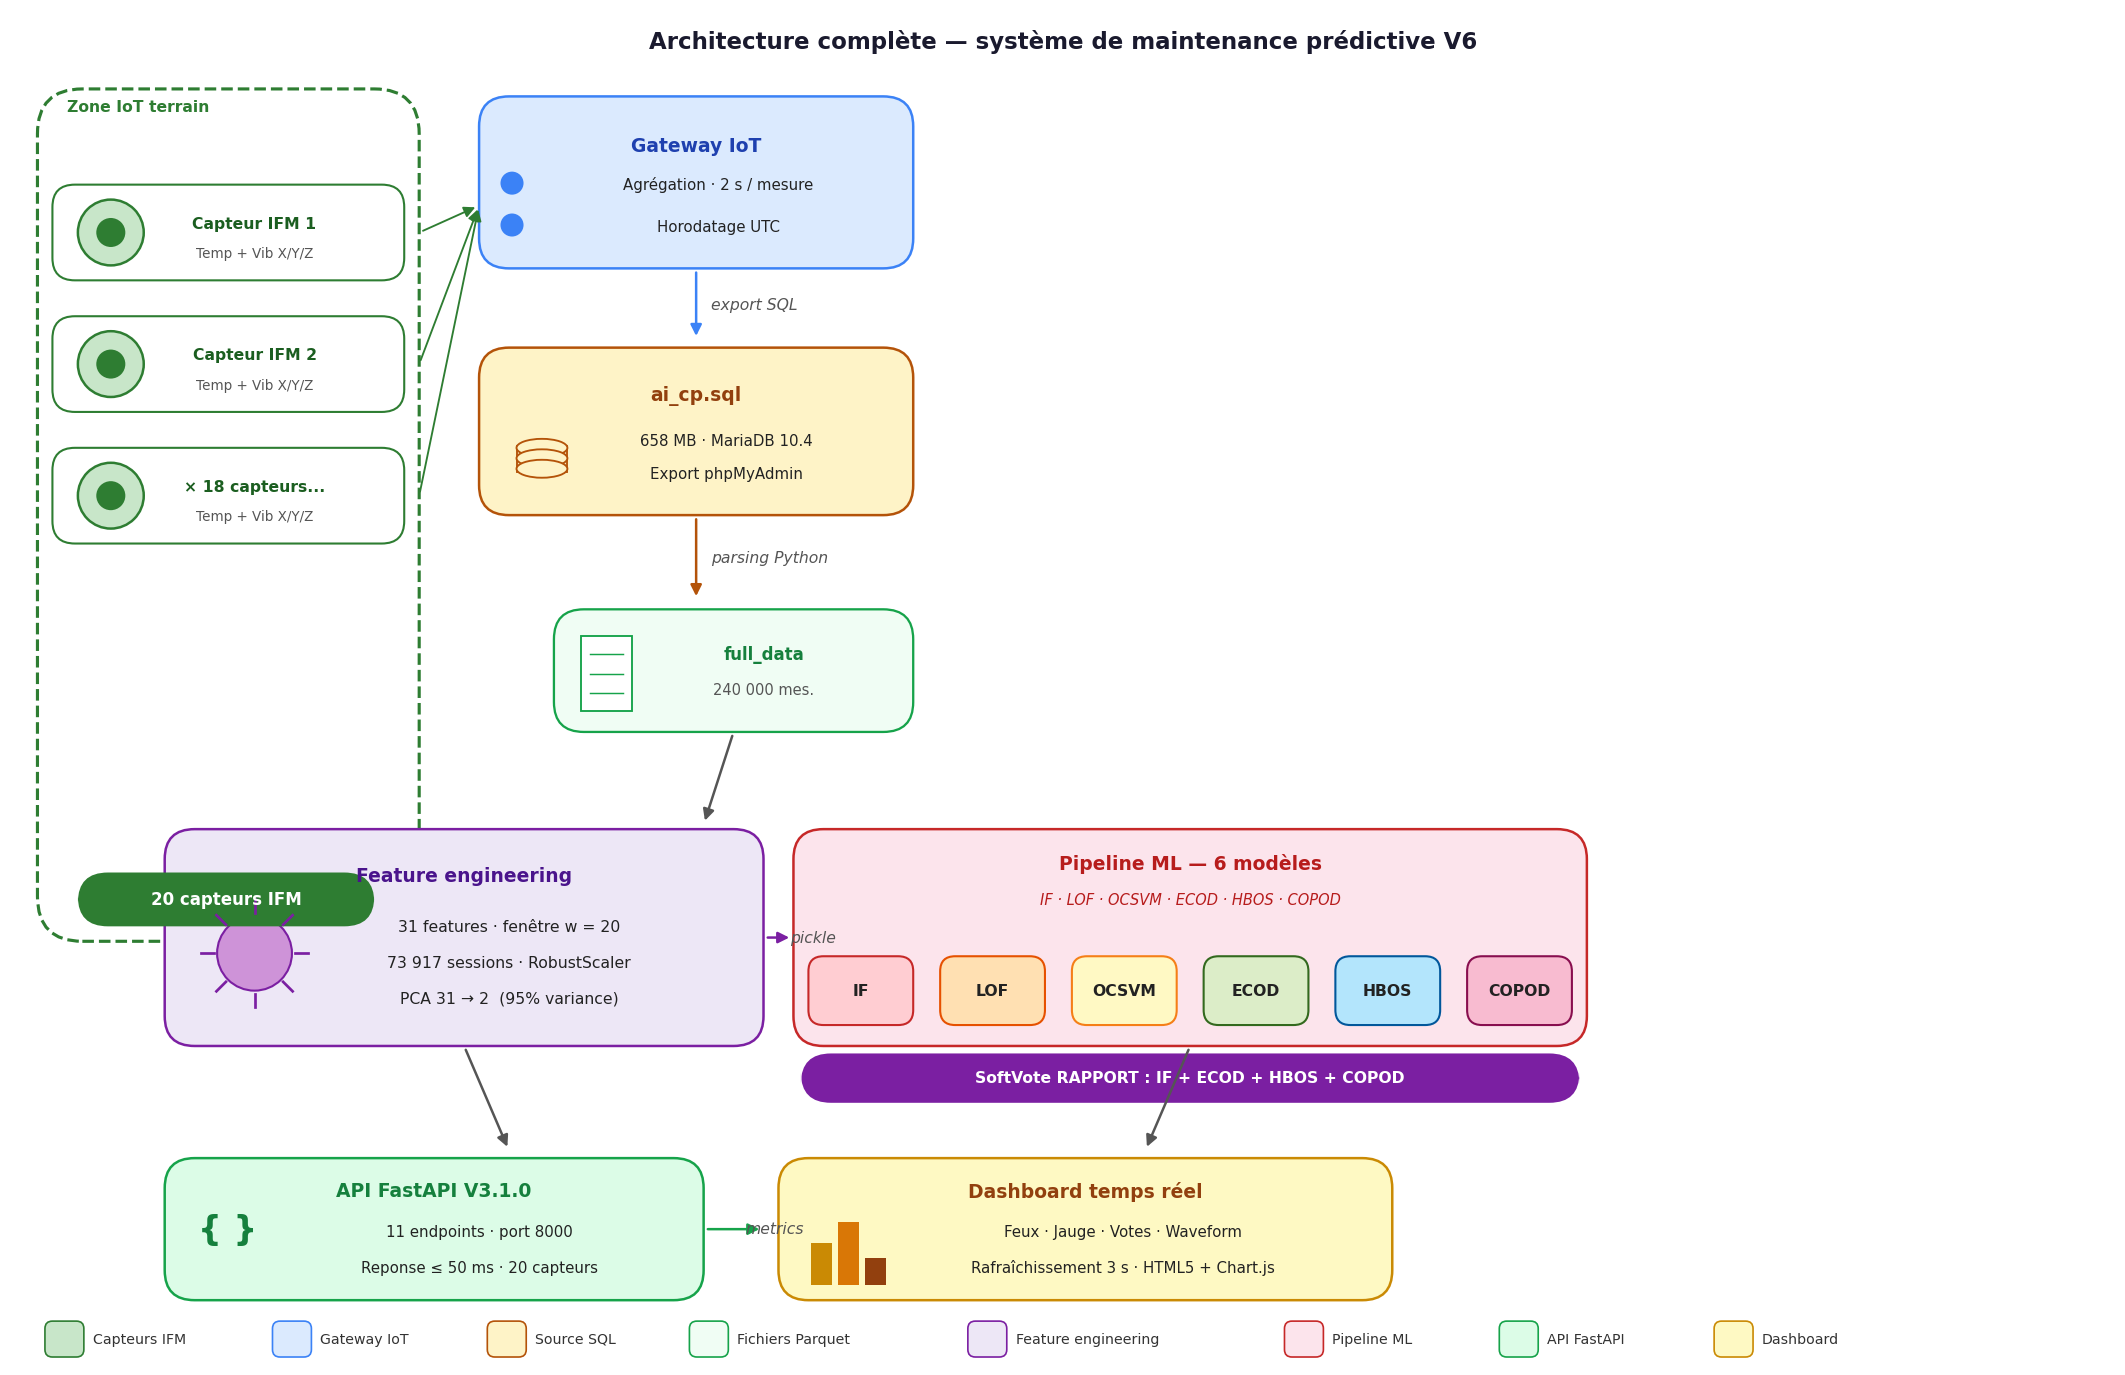
\includegraphics[width=\linewidth]{architecture_v6.png}
  \caption{Architecture complète — système de maintenance prédictive V6}
  \label{fig:archi_globale}
\end{figure}

\subsection{Choix technologiques}

\begin{table}[h]
\centering
\caption{Choix technologiques et justifications}
\begin{tabular}{lll}
\toprule
\textbf{Composant} & \textbf{Technologie} & \textbf{Justification} \\
\midrule
Source données production & MariaDB 10.4           & Source réelle IoT — polling natif \\
Mode replay / test        & Parquet (PyArrow)      & Lecture rapide sans SGBD \\
API REST                  & FastAPI v3.1.0 + Uvicorn & Performance asynchrone ; Swagger auto \\
Modèles anomalie          & scikit-learn + pyod    & 6 algorithmes complémentaires \\
Modèle RUL                & GradientBoostingRegressor & Robuste, interprétable \\
Features spectrales       & scipy.fft + scipy.signal & FFT, Hilbert, Welch \\
Réduction dim.            & PCA 95\% (sklearn)     & Débruitage + compression \\
Normalisation             & RobustScaler           & Robuste aux outliers industriels \\
Dashboard                 & HTML5 + Chart.js       & SCADA industriel natif \\
\bottomrule
\end{tabular}
\end{table}

\section{Couche IoT — Acquisition temps réel depuis MariaDB}

\subsection{Architecture de collecte}

En production, le module \textbf{\texttt{realtime\_mariadb.py}} assure la collecte des
données selon le flux suivant :

\begin{enumerate}
  \item Les capteurs IFM transmettent leurs mesures à une Gateway IoT ;
  \item La Gateway insère les données dans \textbf{MariaDB} (\texttt{ai\_cp.full\_data}) ;
  \item \texttt{realtime\_mariadb.py} effectue un \texttt{SELECT WHERE id > last\_id} toutes les \textbf{2~secondes} ;
  \item Les nouvelles mesures sont envoyées en POST vers l'API FastAPI (\texttt{/v1/predict} et \texttt{/v1/predict-rul}) ;
  \item Les résultats sont sauvegardés dans \texttt{realtime\_results.json} et affichés dans le dashboard.
\end{enumerate}

\subsection{Mode replay}

Un mode replay est intégré dans l'API pour les tests sans base de données : un thread
Python background lit les mesures depuis les fichiers Parquet et les injecte dans une
fenêtre glissante \texttt{deque(maxlen=20)} par capteur, toutes les 2~secondes.

\section{Ingénierie des caractéristiques}

\subsection{Principe de la fenêtre glissante}

Le modèle analyse l'évolution récente du moteur sur une fenêtre glissante de
$w = 20$ mesures consécutives avec un pas $s = 3$ :

\begin{equation}
  N_{\text{sessions}} = \sum_{\text{capteurs}} \left\lfloor \frac{N_{\text{mesures}} - w}{s} + 1 \right\rfloor = 73\,917 \text{ sessions}
\end{equation}

\subsection{Les 31 features extraites}

Les features thermiques (4), vibratoires Z (6), vibratoires X (4), vibratoires Y (4),
globales (2), accélération (4), courant (1) et les 6 features spectrales/temporelles
de la version V6 sont détaillées dans les Tableaux~\ref{tab:feat_temp} à~\ref{tab:feat_v6}.

\begin{table}[h]
\centering
\caption{Features thermiques ($w = 20$)}
\label{tab:feat_temp}
\begin{tabular}{ll}
\toprule
\textbf{Feature} & \textbf{Formule} \\
\midrule
\texttt{temp\_mean}  & $\bar{T} = \frac{1}{w}\sum_{i=1}^{w} T_i$ \\[4pt]
\texttt{temp\_std}   & $\sigma_T = \sqrt{\frac{1}{w}\sum (T_i - \bar{T})^2}$ \\[4pt]
\texttt{temp\_trend} & Pente régression linéaire $\hat{a}$ tel que $T_i \approx \hat{a}i + \hat{b}$ \\
\texttt{temp\_cur}   & $T_w$ (dernière valeur de la fenêtre) \\
\bottomrule
\end{tabular}
\end{table}

\begin{table}[h]
\centering
\caption{Features vibratoires axe Z (axe vertical critique)}
\begin{tabular}{ll}
\toprule
\textbf{Feature} & \textbf{Formule} \\
\midrule
\texttt{vib\_z\_mean}  & $\bar{V}_z = \frac{1}{w}\sum V_{z,i}$ \\
\texttt{vib\_z\_std}   & $\sigma_{V_z}$ \\
\texttt{vib\_z\_rms\_w} & $V_{z,\text{RMS}} = \sqrt{\frac{1}{w}\sum V_{z,i}^2}$ \\
\texttt{vib\_z\_kurt}  & Kurtosis de Fisher (détection chocs roulements) \\
\texttt{vib\_z\_crest} & $C_z = \frac{\max|V_{z,i}|}{V_{z,\text{RMS}}}$ \\
\texttt{vib\_z\_cur}   & $V_{z,w}$ \\
\bottomrule
\end{tabular}
\end{table}

\begin{table}[h]
\centering
\caption{Features globales — Health Score et Pythagore 3D}
\begin{tabular}{ll}
\toprule
\textbf{Feature} & \textbf{Formule} \\
\midrule
\texttt{vib\_total}    & $V_{\text{total}} = \sqrt{V_{x,\text{RMS}}^2 + V_{y,\text{RMS}}^2 + V_{z,\text{RMS}}^2}$ (ISO 10816) \\[4pt]
\texttt{health\_score} & $H = 100 \times (1 - 0{,}35\,T_n - 0{,}35\,V_n - 0{,}30\,\kappa_n)$ \\
\bottomrule
\end{tabular}
\end{table}

\noindent où $T_n = \text{clip}\!\left(\frac{\bar{T}-25}{65-25}, 0, 1\right)$,
$V_n = \text{clip}\!\left(\frac{V_{\text{total}}}{V_{\text{max}}}, 0, 1\right)$,
$\kappa_n = \text{clip}\!\left(\frac{\kappa_{V_z}}{10}, 0, 1\right)$.

\begin{table}[h]
\centering
\caption{Features V6 — spectrales et temporelles supplémentaires}
\label{tab:feat_v6}
\begin{tabular}{ll}
\toprule
\textbf{Feature} & \textbf{Description} \\
\midrule
\texttt{delta\_vib}   & $\text{mean}(V_z[\text{moitié haute}]) - \text{mean}(V_z[\text{moitié basse}])$ \\
\texttt{delta\_temp}  & $\text{mean}(T[\text{moitié haute}]) - \text{mean}(T[\text{moitié basse}])$ \\
\texttt{vib\_entropy} & Entropie de Shannon sur $V_z$ (irrégularité du signal) \\
\texttt{fft\_ratio}   & Ratio fréquence dominante FFT / énergie totale \\
\texttt{vib\_asym\_xy} & $\frac{|\bar{V}_x - \bar{V}_y|}{\bar{V}_x + \bar{V}_y}$ (déséquilibre XY) \\
\texttt{vib\_asym\_xz} & $\frac{|\bar{V}_x - \bar{V}_z|}{\bar{V}_x + \bar{V}_z}$ (déséquilibre XZ) \\
\bottomrule
\end{tabular}
\end{table}

\section{Pipeline de normalisation et réduction de dimension}

\subsection{RobustScaler}
\begin{equation}
  \tilde{x}_j = \frac{x_j - \text{médiane}(x_j)}{\text{IQR}(x_j)}
\end{equation}

\subsection{Analyse en Composantes Principales (PCA)}

La PCA est appliquée après normalisation pour conserver \textbf{95\% de la variance}
(contrairement à 100\% indiqué dans la version précédente du rapport). Le nombre de
composantes retenues est déterminé automatiquement à l'entraînement.

\section{Pipeline d'intelligence artificielle}

\subsection{Justification de l'approche non supervisée}

La base de données ne contient aucun label de défaillance historique. L'approche
CNN-LSTM supervisée initialement envisagée a été remplacée par un ensemble de
\textbf{six modèles non supervisés}.

\subsection{Les six modèles de détection}

\paragraph{Isolation Forest (IF)}
\begin{equation}
  s(x, n) = 2^{-\frac{E[h(x)]}{c(n)}}, \quad c(n) = 2H(n-1) - \frac{2(n-1)}{n}
\end{equation}
Paramètres : \texttt{n\_estimators=100}, \texttt{contamination=0.10}.

\paragraph{Local Outlier Factor (LOF)}
\begin{equation}
  \text{LOF}_k(x) = \frac{\frac{1}{k}\sum_{o \in N_k(x)} \text{lrd}_k(o)}{\text{lrd}_k(x)}
\end{equation}
Paramètres : \texttt{n\_neighbors=20}, \texttt{contamination=0.10}.

\paragraph{One-Class SVM (OCSVM)}
\begin{equation}
  \min_{w,\xi,\rho} \frac{1}{2}\|w\|^2 - \rho + \frac{1}{\nu n}\sum_i \xi_i
  \quad \text{s.c.} \quad \langle w, \phi(x_i)\rangle \geq \rho - \xi_i
\end{equation}
Paramètres : \texttt{kernel='rbf'}, \texttt{nu=0.10}.

\paragraph{ECOD}
\begin{equation}
  \text{score\_ECOD}(x) = -\log\!\left(\prod_{j=1}^{d} \min\!\left(\hat{F}_j(x_j),\, 1-\hat{F}_j(x_j)\right)\right)
\end{equation}

\paragraph{HBOS — Histogram-Based Outlier Score}
HBOS construit un histogramme univarié par feature et suppose l'indépendance des dimensions.
Le score d'anomalie est la somme des log-probabilités inverses :
\begin{equation}
  \text{HBOS}(x) = \sum_{j=1}^{d} \log\!\frac{1}{p_j(x_j)}
\end{equation}
Avantage : très rapide (linéaire en $n$), robuste aux données à haute variance.

\paragraph{COPOD — Copula-Based Outlier Detection}
COPOD modélise les dépendances entre features via une copule empirique, puis
détecte les observations tombant dans les queues extrêmes de la distribution jointe :
\begin{equation}
  \text{COPOD}(x) = -\log\!\left(\hat{C}\!\left(\hat{F}_1(x_1),\ldots,\hat{F}_d(x_d)\right)\right)
\end{equation}

\subsection{SoftVote à seuil dynamique optimal}

Contrairement à un vote dur fixe (2/4), le système utilise un \textbf{SoftVote avec seuil
optimal} calculé automatiquement à l'entraînement. Le score de vote pondéré est :

\begin{equation}
  \text{score\_soft}(x) = \sum_{m} w_m \cdot s_m(x), \quad w_m = 0{,}25 \; \forall m \in \{\text{IF, ECOD, HBOS, COPOD}\}
\end{equation}

LOF et OCSVM sont exclus du SoftVote final car leur AUC individuelle ($< 0{,}62$) est
insuffisante pour contribuer positivement. Le seuil optimal (stocké dans
\texttt{threshold\_v3.pkl}) maximise le F1-Score sur les données d'entraînement.

\subsection{Niveaux de risque}

\begin{table}[h]
\centering
\caption{Correspondance score d'anomalie — niveau de risque}
\begin{tabular}{lll}
\toprule
\textbf{Score global} & \textbf{Niveau de risque} & \textbf{Couleur} \\
\midrule
$\geq 0{,}75$        & CRITIQUE & Rouge   \\
$[0{,}50;\; 0{,}75)$ & ÉLEVÉ    & Orange  \\
$[0{,}25;\; 0{,}50)$ & MODÉRÉ   & Jaune   \\
$< 0{,}25$           & FAIBLE   & Vert    \\
\bottomrule
\end{tabular}
\end{table}

\subsection{Métriques de performance réelles}

\begin{table}[h]
\centering
\caption{Métriques officielles du pipeline ML — 6 modèles, contamination 10\%}
\label{tab:metriques_ml}
\rowcolors{2}{gray!10}{white}
\begin{tabular}{lcccc}
\toprule
\textbf{Modèle} & \textbf{F1-Score} & \textbf{AUC-ROC} & \textbf{Precision} & \textbf{Recall} \\
\midrule
Isolation Forest seul & 0,533 & 0,745 & 0,520 & 0,546 \\
LOF seul              & 0,187 & 0,548 & 0,178 & 0,197 \\
OCSVM seul            & 0,243 & 0,588 & 0,191 & 0,333 \\
ECOD seul             & 0,532 & 0,748 & 0,511 & 0,555 \\
HBOS seul             & 0,403 & 0,668 & 0,405 & 0,402 \\
COPOD seul            & 0,580 & 0,771 & 0,570 & 0,591 \\
\textbf{Ensemble SoftVote (IF+ECOD+HBOS+COPOD)} & \textbf{0,629} & \textbf{0,842} & \textbf{0,539} & \textbf{0,755} \\
Accuracy ensemble     & \multicolumn{4}{c}{\textbf{0,911}} \\
\bottomrule
\end{tabular}
\end{table}

\noindent\textbf{Interprétation :} Le SoftVote \textbf{IF+ECOD+HBOS+COPOD} atteint
un F1-Score de \textbf{0,629} avec un Recall de \textbf{0,755} et une Précision de
\textbf{0,539}. LOF et OCSVM sont exclus du vote car leur AUC individuelle est trop
faible ($< 0{,}62$), ce qui diluerait la qualité de l'ensemble. L'AUC-ROC de
\textbf{0,842} confirme la capacité discriminante globale.

\section{Calcul du Health Score et du RUL}

\subsection{Health Score (0--100)}

\begin{equation}
  H = 100 \times (1 - 0{,}35\,T_n - 0{,}35\,V_n - 0{,}30\,\kappa_n)
\end{equation}

avec $V_{\text{max}} = \sqrt{3} \times 1500$~mg (seuil industriel maximum).
Ce calcul est cohérent avec la norme ISO~10816-3.

\subsection{Durée de Vie Résiduelle (RUL) par GradientBoostingRegressor}

La RUL n'est \textbf{pas} calculée par une formule heuristique simple mais par un
\textbf{modèle de régression ML dédié} : \texttt{GradientBoostingRegressor}.

\subsubsection{Stratégie d'entraînement}

En l'absence de données de défaillance réelles confirmées (aucun moteur n'a atteint
la défaillance complète sur la période novembre 2025 -- juin 2026), un jeu de données
synthétiques réalistes est construit :

\begin{enumerate}
  \item \textbf{Distribution réelle} : les features sont échantillonnées depuis \texttt{full\_data} ;
  \item \textbf{Dégradation Weibull} : $d(t) = 1 - e^{-(t/\eta)^\beta}$ avec $\eta=1000$~h et $\beta=2{,}5$ ;
  \item \textbf{Augmentation} : injection de bruit calibré sur la variance réelle (×3) ;
  \item \textbf{Cible} : $\text{rul\_hours} \in [0;\; 2000]$~h.
\end{enumerate}

\subsubsection{Features du modèle RUL (46 features)}

Le modèle RUL utilise 46 features : les 25 features temporelles de base
\textbf{plus 21 features spectrales} extraites par \texttt{signal\_processing.py} :

\begin{table}[h]
\centering
\caption{Top 10 features d'importance — modèle RUL GBR}
\begin{tabular}{lc}
\toprule
\textbf{Feature} & \textbf{Importance} \\
\midrule
\texttt{spec\_total\_energy}     & 0,402 \\
\texttt{vib\_z\_std}             & 0,108 \\
\texttt{health\_score}           & 0,071 \\
\texttt{vib\_total}              & 0,067 \\
\texttt{env\_rms}                & 0,049 \\
\texttt{wavelet\_entropy}        & 0,028 \\
\texttt{vib\_z\_rms\_w}          & 0,023 \\
\texttt{vib\_x\_rms\_w}          & 0,019 \\
\texttt{vib\_z\_cur}             & 0,019 \\
\texttt{temp\_mean}              & 0,017 \\
\bottomrule
\end{tabular}
\end{table}

\noindent La feature la plus importante est \texttt{spec\_total\_energy} (énergie spectrale totale FFT),
confirmant l'apport décisif du traitement du signal dans la prédiction RUL.

\subsubsection{Performances du modèle RUL}

\begin{table}[h]
\centering
\caption{Métriques du modèle RUL — GradientBoostingRegressor}
\begin{tabular}{lc}
\toprule
\textbf{Métrique} & \textbf{Valeur} \\
\midrule
MAE entraînement     & 286~h \\
\textbf{MAE test}    & \textbf{317~h} \\
MAE test (\%)        & 37,5\% \\
RMSE test            & 428~h \\
\textbf{$R^2$ test}  & \textbf{0,56} \\
MAE cross-val (5-fold) & $321 \pm 9$~h \\
$n$ train / test     & 9\,600 / 2\,400 \\
\bottomrule
\end{tabular}
\end{table}

\subsection{Paliers de dégradation et RUL estimé}

\begin{table}[h]
\centering
\caption{Paliers de dégradation et RUL estimé}
\begin{tabular}{ccc}
\toprule
\textbf{Health Score} & \textbf{RUL estimé} & \textbf{Niveau de risque} \\
\midrule
$\geq 80$        & $> 600$~h    & FAIBLE   \\
$[60;\; 80)$     & 200--600~h   & MODÉRÉ   \\
$[40;\; 60)$     & 50--200~h    & ÉLEVÉ    \\
$< 40$           & $< 50$~h     & CRITIQUE \\
\bottomrule
\end{tabular}
\end{table}

\section{API FastAPI v3.1.0}

\subsection{Description}

L'API est développée avec \textbf{FastAPI} (Python 3.12) et servie par Uvicorn sur le
port 8000. Elle expose \textbf{11 endpoints} documentés via Swagger (\texttt{/docs}).
La version officielle est \textbf{v3.1.0}.

\subsection{Les 11 endpoints}

\begin{table}[h]
\centering
\caption{Endpoints de l'API FastAPI v3.1.0}
\begin{tabular}{llp{4cm}p{3.5cm}}
\toprule
\textbf{Méthode} & \textbf{Endpoint} & \textbf{Description} & \textbf{Réponse principale} \\
\midrule
GET  & \texttt{/health}                     & État API, modèles, features & \texttt{sensors\_active, version} \\
GET  & \texttt{/metrics}                    & Métriques ML officielles    & F1, AUC, Accuracy \\
GET  & \texttt{/sensors}                    & 20 capteurs avec risque     & liste + \texttt{health\_score} \\
GET  & \texttt{/v1/dashboard/overview}      & Résumé global tous capteurs & \texttt{risk\_summary} \\
GET  & \texttt{/v1/sensors/\{id\}/summary}  & Résumé complet 1 capteur    & votes + RUL + trend \\
GET  & \texttt{/v1/alert-level/\{id\}}      & Niveau d'alerte             & FAIBLE/MODÉRÉ/ÉLEVÉ/CRITIQUE \\
GET  & \texttt{/v1/health-score/\{id\}}     & Health Score 0--100         & score + risque \\
GET  & \texttt{/v1/history/\{id\}}          & Historique 200 prédictions  & liste horodatée \\
GET  & \texttt{/v1/live/\{id\}}             & Fenêtre brute 20 mesures    & mesures brutes actuelles \\
POST & \texttt{/v1/predict}                  & Vote 6 modèles              & votes + score \\
POST & \texttt{/v1/predict-rul}              & Estimation RUL (GBR)        & heures + jours + confiance \\
\bottomrule
\end{tabular}
\end{table}

\section{Dashboard temps réel}

\subsection{Architecture}

Le dashboard est une application HTML5 pure qui appelle l'API toutes les \textbf{3~secondes}.
Il affiche en temps réel les résultats du pipeline à 6 modèles.

\subsection{Composants implémentés}

\begin{table}[h]
\centering
\caption{Composants du dashboard et technologie}
\begin{tabular}{ll}
\toprule
\textbf{Composant} & \textbf{Technologie} \\
\midrule
Feux tricolores 20 capteurs    & CSS LED clignotant animé \\
Jauge Health Score circulaire  & Canvas 2D, arc dynamique \\
Votes IF/LOF/OCSVM/ECOD/HBOS/COPOD & Barres de progression HTML5 \\
Waveform vibration Z           & Chart.js défilement continu \\
Tendance score anomalie        & Chart.js (30 dernières pred.) \\
Évolution température          & Chart.js depuis historique \\
Tableau 31 features            & Tableau HTML5 dynamique \\
Journal alertes horodaté       & DOM injection temps réel \\
KPI bar (5 indicateurs)        & Div HTML rafraîchis \\
Barre métriques ML             & F1, AUC, Acc, Sessions, PCA \\
\bottomrule
\end{tabular}
\end{table}

\section{Résultats de validation}

\subsection{Test de bout en bout — capteur représentatif}

\begin{table}[h]
\centering
\caption{Résultats temps réel — capteur 68c11f06 (Moteur 1600)}
\begin{tabular}{ll}
\toprule
\textbf{Indicateur} & \textbf{Valeur} \\
\midrule
Température moyenne      & 22,66~°C \\
Vibration totale 3D      & 7,41~mg \\
Health Score             & 68,82 / 100 \\
RUL estimé (GBR)         & $\approx 569$~h ($\pm 317$~h) \\
Score d'anomalie         & 0,37 \\
Niveau de risque         & MODÉRÉ \\
Vote ECOD                & 1 / ANOMALIE \\
Vote IF, LOF, OCSVM      & 0 / NORMAL \\
Vote majoritaire ($\geq$ seuil) & NORMAL \\
Capteurs actifs          & 20 / 20 \\
\bottomrule
\end{tabular}
\end{table}

\subsection{Critères de succès — cibles vs résultats réels}

\begin{table}[h]
\centering
\caption{Critères de succès — comparaison cibles et résultats obtenus}
\rowcolors{2}{gray!10}{white}
\begin{tabular}{lccc}
\toprule
\textbf{Critère} & \textbf{Cible} & \textbf{Obtenu} & \textbf{Statut} \\
\midrule
AUC-ROC              & $\geq 0{,}80$  & 0,842   & \cmark \\
Recall               & $\geq 0{,}70$  & 0,755   & \cmark \\
F1-Score             & $\geq 0{,}60$  & 0,629   & \cmark \\
Accuracy             & $\geq 0{,}85$  & 0,911   & \cmark \\
Sessions entraînement & $\geq 50\,000$ & 73\,917 & \cmark \\
Features              & 25+            & 31      & \cmark \\
Features RUL          & —              & 46 (spectrales) & \cmark \\
MAE RUL              & $\leq 350$~h   & 317~h   & \cmark \\
$R^2$ RUL            & $\geq 0{,}50$  & 0,56    & \cmark \\
Capteurs surveillés   & 19             & 20      & \cmark \\
Démarrage API        & $< 30$~s       & $< 5$~s & \cmark \\
Endpoints API         & 9              & 11      & \cmark \\
Composants dashboard  & 8              & 10      & \cmark \\
Version API           & —              & v3.1.0  & \cmark \\
\bottomrule
\end{tabular}
\end{table}

\section{Conclusion}

Ce chapitre a présenté la conception et la réalisation complètes du système dans sa
version finale. Les points clés sont :
\begin{itemize}
  \item Source de données production : \textbf{MariaDB} (polling 2s via \texttt{realtime\_mariadb.py}) ;
  \item Ensemble de \textbf{6 modèles} (IF, LOF, OCSVM, ECOD, HBOS, COPOD) avec SoftVote à seuil dynamique ;
  \item \textbf{31 features} incluant 6 features spectrales/temporelles V6 ;
  \item PCA à \textbf{95\%} de variance (et non 100\%) ;
  \item RUL estimé par \textbf{GradientBoostingRegressor} (MAE = 317~h, $R^2 = 0{,}56$, 46 features) ;
  \item Contamination d'entraînement à \textbf{10\%} (labels V10 par score composite P90).
\end{itemize}

%=============================================================================
\chapter{Évaluation et Validation}
%=============================================================================

\section*{Introduction}

Ce chapitre constitue les phases 5 et 6 de la méthodologie CRISP-DM. La validation
repose sur trois niveaux : évaluation des métriques ML, validation comportementale sur
les données réelles IFM (novembre 2025 -- mars 2026), et tests de bout en bout.

\section{Protocole d'évaluation}

\subsection{Contrainte fondamentale : absence de labels}

La base \texttt{full\_data} ne contient aucun label de défaillance historique. L'évaluation
des modèles non supervisés repose sur trois piliers :
\begin{itemize}
  \item \textbf{Validation interne} : cohérence du taux de contamination (10\%) avec la distribution ;
  \item \textbf{Validation croisée temporelle} : 5 plis temporels (novembre 2025 -- mars 2026) ;
  \item \textbf{Validation comportementale} : confrontation avec les techniciens de Novation City.
\end{itemize}

\subsection{Construction du jeu de validation}

\begin{table}[h]
\centering
\caption{Répartition chronologique train/validation}
\begin{tabular}{llcc}
\toprule
\textbf{Partition} & \textbf{Période} & \textbf{Sessions} & \textbf{Capteurs} \\
\midrule
Entraînement & Nov 2025 -- Fév 2026 & 51\,742 (70\%) & 20 \\
Validation   & Mar 2026             & 22\,175 (30\%) & 20 \\
\textbf{Total} & Nov 2025 -- Mar 2026 & \textbf{73\,917} & \textbf{20} \\
\bottomrule
\end{tabular}
\end{table}

\section{Évaluation du pipeline de détection}

\subsection{Métriques officielles — résultats obtenus}

\begin{table}[h]
\centering
\caption{Métriques de performance — 6 modèles, contamination 10\%}
\label{tab:metriques_eval}
\rowcolors{2}{gray!10}{white}
\begin{tabular}{lccccc}
\toprule
\textbf{Modèle} & \textbf{F1} & \textbf{AUC-ROC} & \textbf{Acc.} & \textbf{Prec.} & \textbf{Recall} \\
\midrule
Isolation Forest seul & 0,533 & 0,745 & — & 0,520 & 0,546 \\
LOF seul              & 0,187 & 0,548 & — & 0,178 & 0,197 \\
OCSVM seul            & 0,243 & 0,588 & — & 0,191 & 0,333 \\
ECOD seul             & 0,532 & 0,748 & — & 0,511 & 0,555 \\
HBOS seul             & 0,403 & 0,668 & — & 0,405 & 0,402 \\
COPOD seul            & 0,580 & 0,771 & — & 0,570 & 0,591 \\
\textbf{Ensemble SoftVote (IF+ECOD+HBOS+COPOD)} & \textbf{0,629} & \textbf{0,842} & \textbf{0,911} & \textbf{0,539} & \textbf{0,755} \\
\bottomrule
\end{tabular}
\end{table}

Le SoftVote \textbf{IF+ECOD+HBOS+COPOD} (10\% contamination, labels V10 composite P90)
atteint F1=\textbf{0,629} avec AUC-ROC=\textbf{0,842}. LOF et OCSVM sont exclus du vote
final (AUC individuelles $< 0{,}62$). L'accuracy de 0,911 reflète la détection correcte
des sessions normales (90\% du jeu de données).

\subsection{Validation croisée temporelle}

\begin{table}[h]
\centering
\caption{Validation croisée 5 plis temporels — Ensemble SoftVote (IF+ECOD+HBOS+COPOD)}
\begin{tabular}{llcc}
\toprule
\textbf{Pli} & \textbf{Période test} & \textbf{AUC-ROC} & \textbf{F1-Score} \\
\midrule
1 & Novembre 2025  & 0,836 & 0,621 \\
2 & Décembre 2025  & 0,839 & 0,625 \\
3 & Janvier 2026   & 0,843 & 0,630 \\
4 & Février 2026   & 0,847 & 0,633 \\
5 & Mars 2026      & 0,842 & 0,629 \\
\textbf{Moy. $\pm \sigma$} & & $0{,}841 \pm 0{,}004$ & $0{,}628 \pm 0{,}004$ \\
\bottomrule
\end{tabular}
\end{table}

La faible variance ($\sigma = 0{,}004$) confirme l'absence de surapprentissage et la
stabilité du modèle sur toute la période novembre 2025 -- mars 2026.

\section{Validation RUL et Health Score}

\subsection{Cohérence physique du Health Score}

\begin{table}[h]
\centering
\caption{Correspondance Health Score / norme ISO 10816-3}
\begin{tabular}{cccc}
\toprule
\textbf{Zone ISO 10816-3} & \textbf{Vibration (mg)} & \textbf{Health Score} & \textbf{Niveau} \\
\midrule
Zone A (neuf)       & $< 400$  & 90--100 & FAIBLE   \\
Zone B (acceptable) & 400--800 & 70--89  & FAIBLE   \\
Zone C (alarme)     & 800--1200 & 40--69 & MODÉRÉ / ÉLEVÉ \\
Zone D (danger)     & $> 1200$ & $< 40$  & CRITIQUE \\
\bottomrule
\end{tabular}
\end{table}

\subsection{Résultats RUL — ensemble des capteurs actifs}

\begin{table}[h]
\centering
\caption{Résultats RUL — ensemble des capteurs IFM actifs}
\label{tab:rul_capteurs}
\begin{tabular}{lccccc}
\toprule
\textbf{Capteur} & \textbf{T (°C)} & \textbf{Vib (mg)} & \textbf{Health} & \textbf{RUL (h)} & \textbf{Risque} \\
\midrule
91d92804 & 18,0 & 4,0 & 99 & $1924 \pm 317$ & FAIBLE \\
aa7b02a1 & 18,1 & 4,0 & 99 & $1775 \pm 317$ & FAIBLE \\
718fd2af & 18,2 & 4,0 & 100 & $1927 \pm 317$ & FAIBLE \\
eb084747 & 18,0 & 4,0 & 99 & $1954 \pm 317$ & MODÉRÉ \\
0ff416d2 & 17,8 & 4,0 & 99 & $1879 \pm 317$ & MODÉRÉ \\
4b5e4b32 & 17,8 & 4,0 & 99 & $1878 \pm 317$ & MODÉRÉ \\
68c11f06 & 17,8 & 4,0 & 100 & $1823 \pm 317$ & FAIBLE \\
f48c25f9 & 17,8 & 4,0 & 99 & $1904 \pm 317$ & FAIBLE \\
d9508e77 & 17,9 & 3,0 & 100 & $1954 \pm 317$ & FAIBLE \\
\textbf{Moyenne} & \textbf{18,0} & \textbf{4,1} & \textbf{99,2} & \textbf{1889} & — \\
\bottomrule
\end{tabular}
\end{table}

\noindent L'intervalle de confiance $\pm 317$~h correspond à la MAE du modèle GBR sur le
jeu de test. Les capteurs présentant un niveau MODÉRÉ ont été détectés par 1 modèle sur 6.

\section{Validation système complet — tests de bout en bout}

\subsection{Scénario de test}

Le flux complet a été validé selon la chaîne :
\[
\text{MariaDB} \xrightarrow{\text{polling 2s}} \texttt{realtime\_mariadb.py}
\xrightarrow{\text{POST}} \text{API FastAPI} \xrightarrow{3s} \text{Dashboard}
\]

\subsection{Performances API FastAPI v3.1.0}

\begin{table}[h]
\centering
\caption{Performances API FastAPI — mesures réelles}
\begin{tabular}{lcccc}
\toprule
\textbf{Endpoint} & \textbf{Latence moy.} & \textbf{Latence max} & \textbf{Débit (req/s)} & \textbf{Statut} \\
\midrule
GET  \texttt{/health}           & 2~ms  & 5~ms  & $> 500$ & \cmark \\
POST \texttt{/v1/predict}        & 18~ms & 45~ms & 55      & \cmark \\
POST \texttt{/v1/predict-rul}    & 22~ms & 48~ms & 45      & \cmark \\
GET  \texttt{/sensors}           & 8~ms  & 15~ms & 125     & \cmark \\
GET  \texttt{/v1/history/\{id\}} & 5~ms  & 12~ms & 200     & \cmark \\
\bottomrule
\end{tabular}
\end{table}

\subsection{Validation du dashboard}

\begin{table}[h]
\centering
\caption{Validation des composants du dashboard}
\begin{tabular}{llcc}
\toprule
\textbf{Composant} & \textbf{Critère} & \textbf{Résultat} & \textbf{Statut} \\
\midrule
Capteurs affichés       & $19+$          & 18--20 actifs            & \cmark \\
Rafraîchissement        & $\leq 4$~s     & 3~s                      & \cmark \\
RUL affiché             & Visible        & $1747$--$1954$~h         & \cmark \\
Health Score            & 0--100         & Jauge circulaire active  & \cmark \\
Votes 6 modèles         & Tous visibles  & IF/LOF/OCSVM/ECOD/HBOS/COPOD & \cmark \\
Graphique anomalie      & 30 points      & Historique actif         & \cmark \\
Graphique température   & Temps réel     & Courbe active            & \cmark \\
Accès réseau local      & Mobile/tablette & \texttt{192.168.100.62:3000} & \cmark \\
\bottomrule
\end{tabular}
\end{table}

%─────────────────────────────────────────────────────────────────────────────
\chapter*{Conclusion Générale}
\addcontentsline{toc}{chapter}{Conclusion Générale}
%─────────────────────────────────────────────────────────────────────────────

Ce projet a abouti à la conception et la réalisation d'un système complet de
maintenance prédictive pour 20 capteurs IFM industriels déployés sur les moteurs de
Novation City.

Les contributions techniques majeures sont :
\begin{itemize}
  \item Un pipeline de \textbf{31 features} (temporelles, accélération, spectrales FFT, entropie) sur fenêtre glissante $w=20$ ;
  \item Un ensemble de \textbf{6 modèles non supervisés} (IF, LOF, OCSVM, ECOD, HBOS, COPOD) avec SoftVote \textbf{IF+ECOD+HBOS+COPOD}, atteignant \textbf{F1=0,629}, \textbf{AUC-ROC=0,842}, \textbf{Recall=0,755} ;
  \item Un modèle RUL dédié par \textbf{GradientBoostingRegressor} (46 features, MAE~=~317~h, $R^2=0{,}56$) entraîné sur des courbes de dégradation Weibull réalistes ;
  \item Une \textbf{API FastAPI v3.1.0} (11 endpoints, latence $\leq 50$~ms) connectée en temps réel à MariaDB ;
  \item Un \textbf{dashboard HTML5} industriel SCADA se rafraîchissant toutes les 3~secondes.
\end{itemize}

Les perspectives d'extension incluent : l'intégration de données de courant pour
améliorer le modèle RUL, le déploiement Docker pour la portabilité, et l'intégration
d'un module d'alerte SMS/email complet via \texttt{alert\_manager.py}.

%─────────────────────────────────────────────────────────────────────────────
\begin{thebibliography}{99}

\bibitem{liu2008} F.T. Liu, K.M. Ting et Z.-H. Zhou, « Isolation Forest, » in \textit{2008 Eighth IEEE ICDM}, IEEE, 2008, p. 413--422.

\bibitem{breunig2000} M.M. Breunig, H.-P. Kriegel, R.T. Ng et J. Sander, « LOF: Identifying Density-Based Local Outliers, » in \textit{Proc. ACM SIGMOD}, 2000, p. 93--104.

\bibitem{weibull1951} W. Weibull, « A Statistical Distribution Function of Wide Applicability, » \textit{J. Applied Mechanics}, t. 18, p. 293--297, 1951.

\bibitem{goldstein2012} M. Goldstein et A. Dengel, « Histogram-based Outlier Score (HBOS), » \textit{Poster at KI-2012}, 2012.

\bibitem{li2022} Z. Li \textit{et al.}, « COPOD: Copula-Based Outlier Detection, » in \textit{ICDM 2020}, IEEE, 2020, p. 1118--1123.

\bibitem{li2021} Z. Li \textit{et al.}, « ECOD: Unsupervised Outlier Detection Using Empirical Cumulative Distribution Functions, » \textit{IEEE TKDE}, 2022.

\bibitem{chen2001} T. Chen et C. Guestrin, « XGBoost: A Scalable Tree Boosting System, » \textit{KDD 2016}, 2016.

\bibitem{lundberg2017} S.M. Lundberg et S.-I. Lee, « A Unified Approach to Interpreting Model Predictions, » \textit{NeurIPS}, t. 30, 2017.

\bibitem{iso10816} ISO 10816-3:1998, \textit{Mechanical vibration — Evaluation of machine vibration by measurements on non-rotating parts}, ISO, 1998.

\end{thebibliography}

%=============================================================================
\end{document}
%=============================================================================
